\defverbatim\setusername{%
    \scriptsize
    \verb+git config --global user.name "Max Mustermann"+
    \newline
}
\defverbatim\setusermail{%
    \scriptsize
    \verb+git config --global user.mail "max.mustermann@example.org"+
    \newline
}

\begin{frame}[fragile]
    \frametitle{setting up your environment}
    \only<1>Let git know who you are\ldots
    \begin{lstlisting}
git config --global user.name "Max Mustermann"
git config --global user.mail "max.m@example.org"
    \end{lstlisting}
\end{frame}

\begin{frame}[fragile]
    \frametitle{git config}
    %global vs. local config
    %\begin{itemize}
        %\item global config in \$HOME/.gitconfig
        %\item repository local config .git/config
    %\end{itemize}
    \begin{description}
        \item[aliases] \hfill \\
            \begin{lstlisting}
git config alias.st=git status
            \end{lstlisting}
        \item[highlighting] \hfill \\
            \begin{lstlisting}
git config --global color.ui=always
            \end{lstlisting}
    \end{description}
\end{frame}

\begin{frame}[fragile]
    \frametitle{lets start\ldots}
    \begin{lstlisting}
mkdir my_new_project; cd my_new_project
git init
    \end{lstlisting}
    or\ldots getting local copy of repository that already exist.\\
    \begin{lstlisting}
git clone https://github.com/blastmaster/ta-git_intro.git
    \end{lstlisting}
\end{frame}

\begin{frame}[fragile]
    \frametitle{What is a git repository?}
    \begin{figure}[b]
        \centering
        \begin{tikzpicture}
            \tikzstyle{state} = [ draw,
                node distance = 1.4em,
                drop shadow = {opacity=0.15},
                font = \fontfamily{lmtt}\selectfont\small,
                shape = rectangle,
                rounded corners = .5em,
                minimum width = 7em,
                minimum height = 2em,
                text opacity = 0.75,
                semithick ]
            \tikzstyle{whatis} = [
                node distance = 1.4em,
                left,
                font = \fontfamily{lmtt}\selectfont\tiny]
            \node[state] (remote) {remote};
            \node[state] (repository) [below=of remote] {Local Repository};
            \node[state] (index) [below=of repository] {Staging Area};
            \node[state] (stash) [below=of index] {Stash};
            \node[state] (tree)  [below=of stash] {Working Directory};

            \node[whatis, left] at (remote.west) {Repository on the internet or network.};
            \node[whatis, left] at (repository.west) {Local repository that contains complete history.};
            \node[whatis, left] at (index.west) {Snapshot of the working tree for next commit.};
            \node[whatis, left] at (stash.west) {A place to hide modification if you need a clean workspace.};
            \node[whatis, left] at (tree.west) {The direcotries and files on your filesystem.};
        \end{tikzpicture}
    \end{figure}
\end{frame}

\begin{frame}
    \frametitle{Staging files}
    \begin{figure}[b]
        \centering
        \begin{tikzpicture}
            \tikzstyle{state} = [ draw,
                node distance = 1.4em,
                drop shadow = {opacity=0.15},
                font = \fontfamily{lmtt}\selectfont\small,
                shape = rectangle,
                rounded corners = .5em,
                minimum width = 7em,
                minimum height = 2em,
                text opacity = 0.75,
                semithick ]
            \tikzstyle{whatis} = [
                node distance = 1.4em,
                font = \fontfamily{lmtt}\selectfont\tiny]
            \node[state] (index) {Staging Area};
            \node[state] (tree)  [below=of index] {Working Directory}
                edge [->, out=0, in=0] node[whatis, right] {git add <filename>} (index)
                edge [<-, out=180, in=180] node[whatis, left] {git reset HEAD <filename>} (index);
        \end{tikzpicture}
    \end{figure}
\end{frame}

\begin{frame}
    \frametitle{Stashing}
    \begin{figure}[b]
        \centering
        \begin{tikzpicture}
            \tikzstyle{state} = [ draw,
                node distance = 1.4em,
                drop shadow = {opacity=0.15},
                font = \fontfamily{lmtt}\selectfont\small,
                shape = rectangle,
                rounded corners = .5em,
                minimum width = 7em,
                minimum height = 2em,
                text opacity = 0.75,
                semithick ]
            \tikzstyle{whatis} = [
                node distance = 1.4em,
                font = \fontfamily{lmtt}\selectfont\tiny]
            \node[state] (stash) [below=of index] {Stash};
            \node[state] (tree)  [below=of stash] {Working Directory}
                edge [->, out=0, in=0] node [whatis, right] {git stash} (stash)
                edge [<-, out=180, in=180] node [whatis, left] {git apply} (stash);
        \end{tikzpicture}
    \end{figure}
\end{frame}


\begin{frame}
    \frametitle{commiting changes}
    \begin{figure}[b]
        \centering
        \begin{tikzpicture}
            \tikzstyle{state} = [ draw,
                node distance = 1.4em,
                drop shadow = {opacity=0.15},
                font = \fontfamily{lmtt}\selectfont\small,
                shape = rectangle,
                rounded corners = .5em,
                minimum width = 7em,
                minimum height = 2em,
                text opacity = 0.75,
                semithick ]
            \tikzstyle{whatis} = [
                node distance = 1.4em,
                font = \fontfamily{lmtt}\selectfont\tiny]
            \node[state] (repository)  {local repository};
            \node[state] (index) [below=of repository] {Staging Area}
                edge [->, out=0, in=0] node [whatis, right] {git commit} (repository);
            \node[state] (tree)  [below=of stash] {Working Directory}
                edge [<-, out=180, in=180] node [whatis, left] {git checkout <commitid>} (repository)
                edge [->, out=0, in=0] node[whatis, right] {git add <filename>} (index);
        \end{tikzpicture}
    \end{figure}
\end{frame}

\begin{frame}
    \frametitle{version control is local}
    \begin{figure}[b]
        \centering
        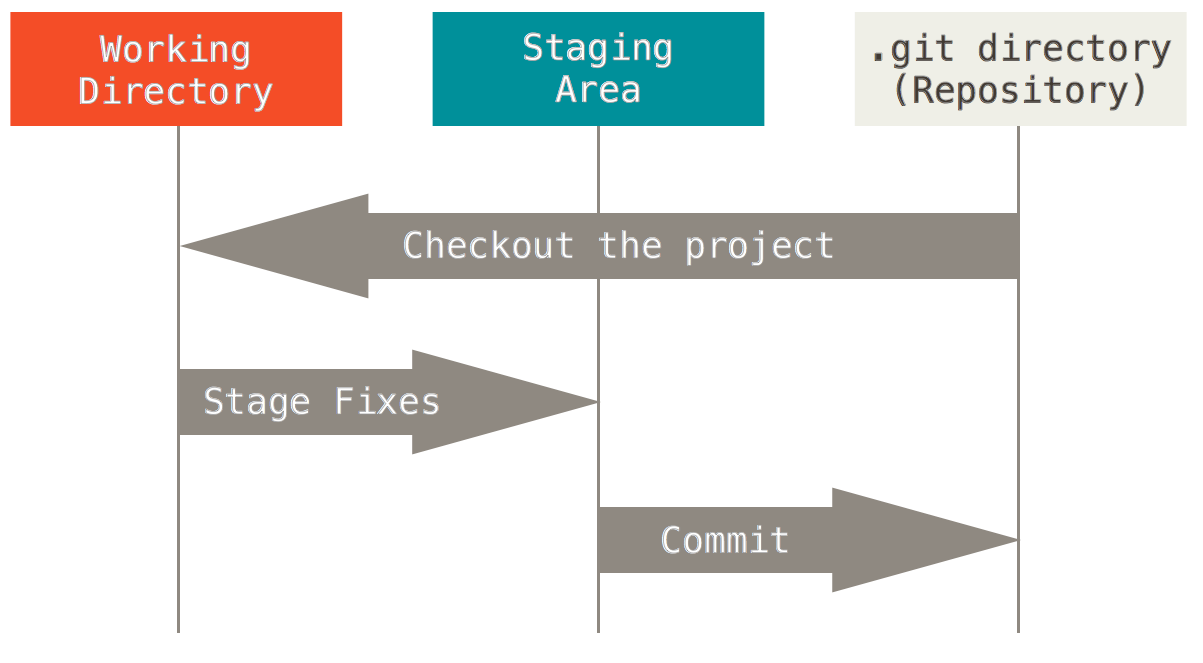
\includegraphics[width=0.9\textwidth]{../img/three_states.png}
    \end{figure}
    % TODO add reference
    % http://www.git-scm.com/book/en/v2/book/01-introduction/images/areas.png
\end{frame}

\begin{frame}
    \frametitle{Lifecycle of our files}
    \begin{figure}[b]
        \centering
            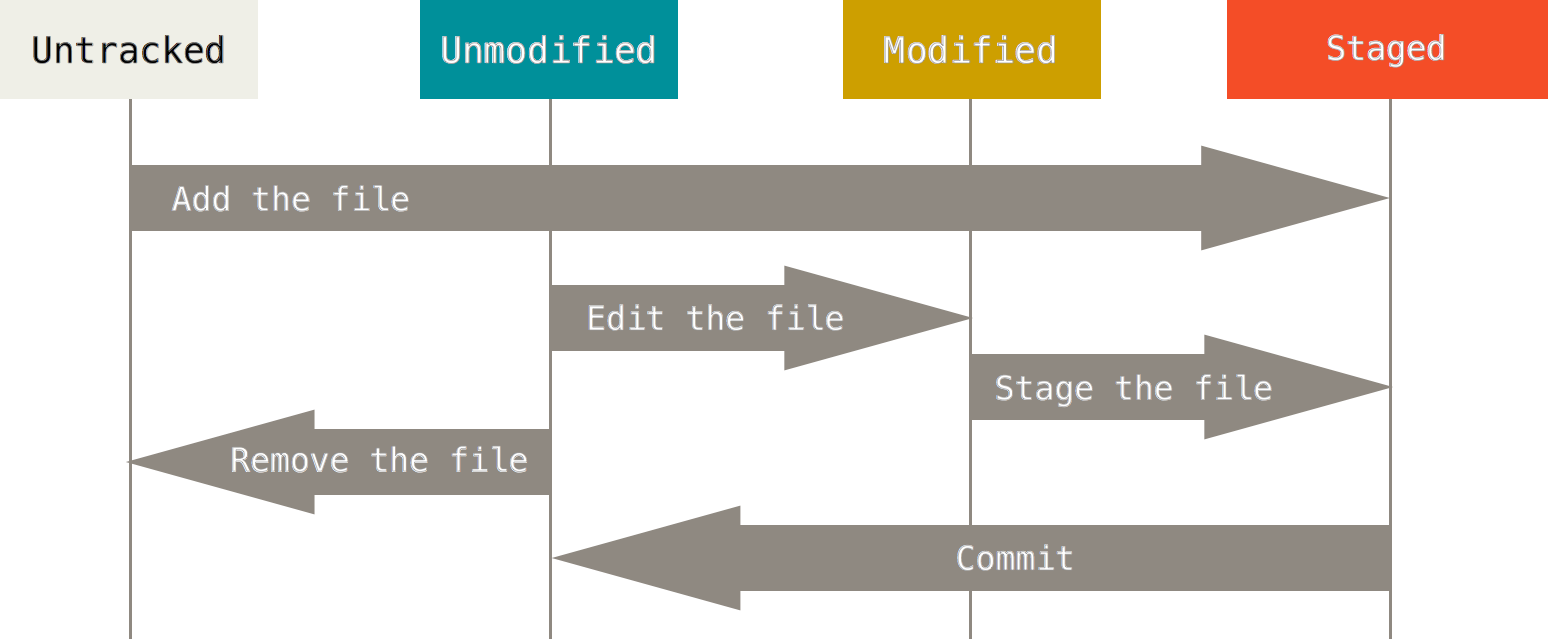
\includegraphics[width=\textwidth]{../img/file_lifecycle.png}
    \end{figure}
    % TODO add reference
    % http://www.git-scm.com/book/en/v2/Git-Basics-Recording-Changes-to-the-Repository
\end{frame}

\begin{frame}
    \frametitle{remote}
    \begin{figure}[b]
        \centering
        \begin{tikzpicture}
            \tikzstyle{state} = [ draw,
                node distance = 1.4em,
                drop shadow = {opacity=0.15},
                font = \fontfamily{lmtt}\selectfont\small,
                shape = rectangle,
                rounded corners = .5em,
                minimum width = 7em,
                minimum height = 2em,
                text opacity = 0.75,
            semithick ]
            \tikzstyle{whatis} = [
                node distance = 1.4em,
                font = \fontfamily{lmtt}\selectfont\tiny]
                \node[state] (remote) {remote: origin};
                \node[state] (working) [below=of remote] {local repository}
                edge [<-, in=0, out=0]  node[whatis, right] {git pull origin master} (remote)
                edge [->, in=180, out=180] node[whatis, left] {git push origin master} (remote);
        \end{tikzpicture}
        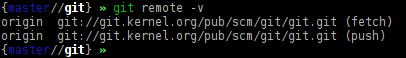
\includegraphics[width=\textwidth]{../img/show_remote.png}
    \end{figure}
\end{frame}


\defverbatim\myadd{%
    \scriptsize
    \verb+git remote add github git@github.com:username/repo.git+
    \newline
}

\begin{frame}[fragile]
    \frametitle{adding a remote}
    \myadd
    \begin{figure}
        \centering
        \begin{tikzpicture}
            \tikzstyle{state} = [ draw,
                node distance = 1.4em,
                drop shadow = {opacity=0.15},
                font = \fontfamily{lmtt}\selectfont\small,
                shape = rectangle,
                rounded corners = .5em,
                minimum width = 7em,
                minimum height = 2em,
                text opacity = 0.75,
            semithick ]
            \tikzstyle{whatis} = [
                node distance = 2.4em,
                font = \fontfamily{lmtt}\selectfont\tiny]
                \node[state] (remote) {remote: origin};
                \node[state] (remote2) [right=of remote] {remote: github};
                \node[state] (working) [below=of remote, xshift=1.25cm] {local copy}
                edge [<->, in=180, out=180] node[whatis, left, align=center] {
                    git pull origin master \\
                git push origin master} (remote)
                edge [<->, in=0, out=0] node[whatis, right, align=center] {git pull github master \\
                git push github master} (remote2);
        \end{tikzpicture}
    \end{figure}
\end{frame}

\defverbatim\mytag{%
    \scriptsize
    \verb+git tag -a v0.1 A+
    \newline
}

\begin{frame}
    \frametitle{Tags}
    Tags are like bookmarks on commits.
    \begin{figure}[b]
        \centering
        \begin{tikzpicture}
            \gitDAG[grow right sep = 2em]
            {
                A -- B -- C
            };
            \gitbranch
            {master}
            {above=of C}
            {C}
            \gitHEAD
            {above=of master}
            {master}
        \end{tikzpicture}
        \caption{lets create a tag for commit A}
    \end{figure}
\end{frame}

\begin{frame}
    \frametitle{Tags - Syntax}
    \begin{description}
        \item[create tag] git tag -a <commitid>
        \item[delete tag] git tag -d <tagname>
        \item[filter tag] git tag -l <pattern>
    \end{description}
\end{frame}

\begin{frame}[fragile]
    \frametitle{Tags}
    \mytag
    \begin{figure}[b]
        \centering
        \begin{tikzpicture}
            \gitDAG[grow right sep = 2em]
            {
                A -- B -- C
            };
            \gitbranch {master}
            {above=of C}
            {C}
            \gittag
            [v0p1]
            {v0.1}
            {above=of A}
            {A}
            \gitHEAD
            {above=of master}
            {master}
        \end{tikzpicture}
        \caption{our brand new tag!}
    \end{figure}
\end{frame}

\begin{frame}
    \frametitle{Branching}
    \begin{figure}[b]
        \centering
        \begin{tikzpicture}
            \gitDAG[grow right sep = 2em]
            {
                A -- B -- C
            };
            \gitbranch {master}
            {above=of C}
            {C}
            \gittag
            [v0p1]
            {v0.1}
            {above=of A}
            {A}
            \gitHEAD
            {above=of master}
            {master}
        \end{tikzpicture}
        \caption{lets create a new branch}
    \end{figure}
\end{frame}

\begin{frame}
    \frametitle{Branch Syntax}
    \begin{description}
        \item[create new branch] \hfill \\
            \begin{itemize}
                \item git branch <branchname>
                \item git checkout -b <branchname>
            \end{itemize}
        \item[delete branch] \hfill \\
            \begin{itemize}
                \item git branch -d <branchname>
            \end{itemize}
    \end{description}
\end{frame}

\begin{frame}
    \frametitle{Branching}
    \begin{figure}[b]
        \centering
        \begin{tikzpicture}
            \gitDAG[grow right sep = 2em]
            {
                A -- B -- {
                    C,
                    D -- E,
                }

            };
            \gitbranch {master}
            {above=of C}
            {C}
            \gittag
            [v0p1]
            {v0.1}
            {above=of A}
            {A}
            \gitbranch
            {feature X}
            {above=of E}
            {E}
            \gitHEAD
            {above=of master}
            {master}
        \end{tikzpicture}
        \caption{lets create a new branch}
    \end{figure}
\end{frame}

\begin{frame}
    \frametitle{Rebasing}
    \begin{figure}
        \centering
        \begin{tikzpicture}
            \gitDAG[grow right sep = 2em]
            {
                A -- B -- {
                    C,
                    D -- E,
                }
            };
            \gittag
            [v0p1]
            {v0.1}
            {above=of A}
            {A}
            \gitremotebranch
            [origmaster]
            {origin/master}
            {above=of C}
            {C}
            \gitbranch
            {master}
            {above=of E}
            {E}
            \gitHEAD
            {above=of master}
            {master}
        \end{tikzpicture}
    \end{figure}
\end{frame}

\begin{frame}
    \frametitle{Rebasing}
    \begin{figure}
        \centering
        \begin{tikzpicture}
            \gitDAG[grow right sep = 2em] {
                A -- B -- {
                    C -- D' -- E',
                    {[nodes=unreachable] D -- E},
                }
            };
            \gittag
            [v0p1]
            {v0.1}
            {above=of A}
            {A}
            \gitremotebranch
            [origmaster]
            {origin/master}
            {above=of C}
            {C}
            \gitbranch
            {master}
            {above=of E'}
            {E'}
            \gitHEAD
            {above=of master}
            {master}
        \end{tikzpicture}
    \end{figure}
\end{frame}

% demonstrate merging of two branches
\begin{frame}
    \frametitle{merging}
    \begin{figure}[b]
        \centering
        \begin{tikzpicture}
            \gitDAG[grow right sep = 2em]
            {
                A -- B -- {
                    C,
                    D -- E,
                }
            };
            \gitbranch
            {master}
            {above=of C}
            {C}
            \gitbranch
            {feature X}
            {above=of E}
            {E}
            \gitHEAD
            {above=of feature X}
            {feature X}
        \end{tikzpicture}
        \caption{Before\ldots}
    \end{figure}
\end{frame}

\begin{frame}
    \frametitle{merging}
    \begin{figure}[b]
        \centering
        \begin{tikzpicture}
            \gitDAG[grow right sep = 2em]
            {
                A -- B --{
                C,
                    {D -- E},
                } -- E'
            };
            \gitbranch
            {master}
            {above=of E'}
            {E'}
            \gitbranch
            {feature X}
            {below=of E}
            {E}
            \gitHEAD
            {above=of master}
            {master}
        \end{tikzpicture}
        \caption{after: \texttt{git merge feature X}}
    \end{figure}
\end{frame}

\begin{frame}
    \frametitle{follow the changes}
    \begin{description}
        \item[what:] git diff [-\,-staged]
        \item[when:] git log
        \item[who:] git blame
    \end{description}
\end{frame}

\begin{frame}
    \frametitle{Reference}
    \begin{itemize}
        \item \url{http://www.git-scm.com/docs} % reference
        \item \url{http://www.git-scm.com/book/en/v2} % book
        \item \url{https://sandofsky.com/blog/git-workflow.html} % workflow
        \item \url{http://ndpsoftware.com/git-cheatsheet.html} % cheatcheet
    \end{itemize}
\end{frame}
